%% For double-blind review submission, w/o CCS and ACM Reference (max submission space)
% \documentclass[sigplan,10pt,review,anonymous]{acmart}\settopmatter{printfolios=true,printccs=false,printacmref=false}
\documentclass[sigplan,10pt,review]{acmart}\settopmatter{printfolios=true,printccs=false,printacmref=false}
%% For double-blind review submission, w/ CCS and ACM Reference
%\documentclass[acmsmall,review,anonymous]{acmart}\settopmatter{printfolios=true}
%% For single-blind review submission, w/o CCS and ACM Reference (max submission space)
%\documentclass[acmsmall,review]{acmart}\settopmatter{printfolios=true,printccs=false,printacmref=false}
%% For single-blind review submission, w/ CCS and ACM Reference
%\documentclass[acmsmall,review]{acmart}\settopmatter{printfolios=true}
%% For final camera-ready submission, w/ required CCS and ACM Reference
% \documentclass[acmsmall]{acmart}\settopmatter{}


%% Journal information
%% Supplied to authors by publisher for camera-ready submission;
%% use defaults for review submission.
\acmJournal{PACMPL}
\acmVolume{1}
\acmNumber{CONF} % CONF = POPL or ICFP or OOPSLA
\acmArticle{1}
\acmYear{2018}
\acmMonth{1}
\acmDOI{} % \acmDOI{10.1145/nnnnnnn.nnnnnnn}
\startPage{1}

%% Copyright information
%% Supplied to authors (based on authors' rights management selection;
%% see authors.acm.org) by publisher for camera-ready submission;
%% use 'none' for review submission.
\setcopyright{none}
%\setcopyright{acmcopyright}
%\setcopyright{acmlicensed}
%\setcopyright{rightsretained}
%\copyrightyear{2018}           %% If different from \acmYear

%% Bibliography style
\bibliographystyle{ACM-Reference-Format}
%% Citation style
%% Note: author/year citations are required for papers published as an
%% issue of PACMPL.
% \citestyle{acmauthoryear}   %% For author/year citations


%%%%%%%%%%%%%%%%%%%%%%%%%%%%%%%%%%%%%%%%%%%%%%%%%%%%%%%%%%%%%%%%%%%%%%
%% Note: Authors migrating a paper from PACMPL format to traditional
%% SIGPLAN proceedings format must update the '\documentclass' and
%% topmatter commands above; see 'acmart-sigplanproc-template.tex'.
%%%%%%%%%%%%%%%%%%%%%%%%%%%%%%%%%%%%%%%%%%%%%%%%%%%%%%%%%%%%%%%%%%%%%%


%% Some recommended packages.
\usepackage{booktabs}   %% For formal tables:
                        %% http://ctan.org/pkg/booktabs
\usepackage{subcaption} %% For complex figures with subfigures/subcaptions
                        %% http://ctan.org/pkg/subcaption
\usepackage{xcolor}
\usepackage{listings}
\lstset{
  basicstyle=\fontsize{9}{10}\selectfont\ttfamily,
  numbers=left,
  numberstyle= \tiny,
  keywordstyle= \color{ blue!70},
  commentstyle= \color{red!50!green!50!blue!50},
  frame=single,
  rulesepcolor= \color{ red!20!green!20!blue!20} ,
  escapeinside=``,
  xleftmargin=1.5em,xrightmargin=0em, aboveskip=1em,
  framexleftmargin=2em,
  showstringspaces=false,
  showtabs=false,
  breaklines=true
}
\lstdefinelanguage{Solidity}
{
  morekeywords={contract, mapping, address, uint, private, function, public, if, payable},
  morecomment=[l]{//},
  morestring=[b]"
}


\usepackage{multicol}
\usepackage{multirow}
\usepackage{lipsum}
\usepackage{mathtools}
\usepackage{cuted}

\usepackage{amsmath}
\usepackage{extpfeil}
\usepackage{mathpartir}
\usepackage[mathscr]{eucal}

\usepackage{hyperref}
\usepackage{cleveref}
\crefformat{section}{\S#2#1#3} % see manual of cleveref, section 8.2.1
\crefformat{subsection}{\S#2#1#3}
\crefformat{subsubsection}{\S#2#1#3}

\usepackage{algorithm}
\usepackage{algorithmicx}
\usepackage{algpseudocode}
\renewcommand{\algorithmicrequire}{\textbf{Input:}}
\renewcommand{\algorithmicensure}{\textbf{Output:}}

\newcommand{\todo}[1]{\textcolor{red}{[TODO: #1]}}

\begin{document}

%% Title information
\title[Network Fusion through CDRP Model Decomposition and Assembly]{Network Fusion through CDRP Model\\ Decomposition and Assembly}         %% [Short Title] is optional;
%% when present, will be used in
%% header instead of Full Title.
%\titlenote{ }             %% \titlenote is optional;
%% can be repeated if necessary;
%% contents suppressed with 'anonymous'
%\subtitle{Subtitle}                     %% \subtitle is optional
%\subtitlenote{with subtitle note}       %% \subtitlenote is optional;
%% can be repeated if necessary;
%% contents suppressed with 'anonymous'


%% Author information
%% Contents and number of authors suppressed with 'anonymous'.
%% Each author should be introduced by \author, followed by
%% \authornote (optional), \orcid (optional), \affiliation, and
%% \email.
%% An author may have multiple affiliations and/or emails; repeat the
%% appropriate command.
%% Many elements are not rendered, but should be provided for metadata
%% extraction tools.

\author{Zhongye Wang}
% \authornote{Supervised by Qinxiang Cao, Shanghai Jiao Tong University, John Hopcroft Center for Computer Science.}          %% \authornote is optional;
%% can be repeated if necessary
%\orcid{nnnn-nnnn-nnnn-nnnn}             %% \orcid is optional
\affiliation{
	%\position{Position2b}
	%\department{Department2b}             %% \department is recommended
	\institution{Shanghai Jiao Tong University}           %% \institution is required
	%\streetaddress{Street3b Address2b}
	%\city{City2b}
	%\state{State2b}
	%\postcode{Post-Code2b}
	%\country{Country2b}                   %% \country is recommended
}
% \email{wangzhongye1110@sjtu.edu.cn}          %% \email is recommended

\author{Yichen Xie}
% \authornote{Supervised by Qinxiang Cao, Shanghai Jiao Tong University, John Hopcroft Center for Computer Science.}          %% \authornote is optional;
%% can be repeated if necessary
%\orcid{nnnn-nnnn-nnnn-nnnn}             %% \orcid is optional
\affiliation{
	%\position{Position2b}
	%\department{Department2b}             %% \department is recommended
	\institution{Shanghai Jiao Tong University}           %% \institution is required
	%\streetaddress{Street3b Address2b}
	%\city{City2b}
	%\state{State2b}
	%\postcode{Post-Code2b}
	%\country{Country2b}                   %% \country is recommended
}
% \email{}          %% \email is recommended

\author{Xinyu Zhan}
% \authornote{Supervised by Qinxiang Cao, Shanghai Jiao Tong University, John Hopcroft Center for Computer Science.}          %% \authornote is optional;
%% can be repeated if necessary
%\orcid{nnnn-nnnn-nnnn-nnnn}             %% \orcid is optional
\affiliation{
	%\position{Position2b}
	%\department{Department2b}             %% \department is recommended
	\institution{Shanghai Jiao Tong University}           %% \institution is required
	%\streetaddress{Street3b Address2b}
	%\city{City2b}
	%\state{State2b}
	%\postcode{Post-Code2b}
	%\country{Country2b}                   %% \country is recommended
}
% \email{}          %% \email is recommended



%% Abstract
%% Note: \begin{abstract}...\end{abstract} environment must come
%% before \maketitle command
\begin{abstract}
  The abstract \dots
\end{abstract}


%% 2012 ACM Computing Classification System (CSS) concepts
%% Generate at 'http://dl.acm.org/ccs/ccs.cfm'.

%% End of generated code


%% Keywords
%% comma separated list
\keywords{}  %% \keywords are mandatory in final camera-ready submission


%% \maketitle
%% Note: \maketitle command must come after title commands, author
%% commands, abstract environment, Computing Classification System
%% environment and commands, and keywords command.
\maketitle

\section{Introduction}
\label{sec:intro}
The introduction \dots

\begin{figure}[h]
    \centering
    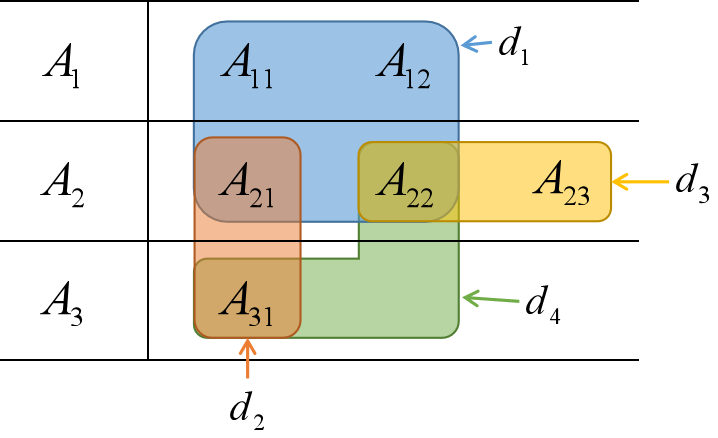
\includegraphics[width=0.75\linewidth]{fig/formulation_example.png}
    \caption{An Example Assembly Problem}
    \label{fig:assemble-example-venn}
\end{figure}

Figure~\ref{fig:assemble-example-venn} shows an example of the assembly problem of our interest.
The original dataset contains 3 classes $A_1, A_2$, and $A_3$, and we are able to decompose each into some subclasses, e.g., $A_1$ is decomposed into two subclasses of samples $A_{11}$ and $A_{12}$.
There are 4 binary classifiers, each determines whether a sample belongs to the union of some subclasses marked with boxes, e.g., $d_1$ determines whether a sample belongs to the union of $\{A_{11}, A_{12}, A_{21}, A_{22}\}$.
We can use classifiers $d_1, d_2, d_3$ and set operations for the classification task:
\begin{itemize}
	\item $d_1 - (d_2 + d_3)$ determines samples belong to $A_1$;
	\item $d_1 \cdot d_2 + d_3$ determines samples belong to $A_2$;
	\item $d_2 - d_1$ determines samples belong to $A_3$.
\end{itemize}
For the partial classification task of class $A_3$, it suffices to use only $d_2$ and $d_4$ and their intersection $d_2 \cdot d_4$ to determine samples in $A_3$.

\subsection{Our Work}

\section{The General Assembly Framework}
\label{sec:assembly}
In this section, we give the general framework to assemble multiple classifiers into one that performs complex classification tasks.
The classification task only need to cover a given set of labels, and we do not need to distinguish the remaining dummy classes.
We also propose an heuristic search algorithm to find a feasible solution to the assembly problem.

We only consider the general case of such assembly in this section, while we specialize the assembly problem w.r.t. input composed of CDRP models in \cref{sec:cdrp}.
The assembly problem can be easily extended to general classifier input, but we only discuss the case for binary classifier input for simplicity.

\subsection{The Assembly Problem}
\label{sec:assemble-problem}
We first formulate the problem by defining the input of an assembly problem and the output it requires.

The input have the following components:
\begin{itemize}
	\item $L$ class labels, denoted $\{l_j\}$
	\item $N$ subclasses in total \begin{itemize}
		\item $M$ target subclasses, denoted $\mathcal{A} = \{A_i\}$
		\item $N-M$ dummy subclasses, denoted $\bar{\mathcal{A}} = \{A_i\}$
	\end{itemize}
	\item $g(A_i) := l_j$ the partial map from $A_i$ to class label $l_j$
	\item $K$ classifiers, denoted $\mathcal{D} = \{d_j\}$
	\item $f(A_i, d_j) := 0, 1$ the classifier certificate function that $A_i$ is classified positive in classifier $d_j$
	\item $score(d_j)$ the performance score of classifier $d_j$
	\item $k$ the maximum number of classifier to use
\end{itemize}

The original dataset consists of $L$ classes with different labels.
Some prior knowledge allows us to decompose the dataset into $N$ subclasses of samples.
A subclass is the unit sample group we will consider in the assembly problem, and for a subclass to be \textit{consistent}, we assume all samples in a subclass have the sample label given by the partial map $g$.
Since we are only interested in a subset of labels, we group all $M$ target subclasses having these labels into $\mathcal{A}$
The rest $N-M$ subclasses are dummy ones.

We are given $K$ binary classifiers with domains of the entire dataset.
All samples in a subclass $A_i$ should be assigned the same 0-1 label by a classifier $d_j$, which is determined by the certificate function $f$.
To extend the assembly problem to general classifier inputs, we only need to change the certificate function $f$ for classifiers to allow return values from a set of multiple symbols.
The cardinality of $f$'s range should be $n$ for an $n$-classifier assembly problem.
For example, a ternary classifier assembly problem needs the certificate function to produce three possible symbols, i.e., $|range(f)| = 3$.

For each classifier, we also know its performance score, which could be its accuracy, its model complexity, or both.
There is a constraint for a problem instance that we can only use up to $k$ classifiers to assemble the final classifier.

The solution to the problem instance should contain:
\begin{itemize}
	\item $D \subset \mathcal{D}$ a set of $m$ classifiers \textit{distinguishing} all $M$ target subclasses s.t. $m < k$
	\item $score(D)$ the overall performance of the classifier set
\end{itemize}

\todo{The overal performance score.}

We define the concept of \textit{distinguishing} as follows.
\begin{definition}
	A set of classifiers covers $M$ target subclasses iff. given any sample, the joint classifier can determine whether it \textit{solely} belongs to \begin{enumerate}
		\item a subset (with consistent labels) of the $M$ target subclasses, or,
		\item the rest dummy subclasses $\bar{\mathcal{A}}$.
	\end{enumerate}
\end{definition}
In other word, the classifier should uniquely determine whether a sample have which of the target labels or the dummy label.

We start with analyzing the intractability of the problem.
\begin{theorem}
	The assembly problem is an NP problem.
\end{theorem}
\begin{proof}
We prove the theorem by giving a polynomial algorithm for the certificate problem.

Given a certificate $D \subset \mathcal{D}$, we encode each subclass with a binary string $s$ of length $k$, where the $j$-th element for the $i$ subclass is $f(A_i, d_j)$ ($d_j \in D$).
This step takes $O(Nk) = O(NK)$ time.
The algorithm returns $yes$ iff. \begin{enumerate}
	\item No two subclasses in $\mathcal{A}$ share the same encoding but have different labels, and,
	\item No subclass in $\mathcal{A}$ shares the same encoding with any subclass in $\bar{\mathcal{A}}$.
\end{enumerate}
Otherwise, it returns $no$.
This step takes $O(N)$ if we use hash table to record the occurrence of encoded strings.

% \begin{algorithm}[h]
% 	\caption{}
% 	\begin{algorithmic}
% 		\Require A assembly problem instance $k$; a certificate $D \subset \mathcal{D}$.
% 		\Ensure Whether problem instance $k$ is solvable.
% 		\State initialize a hash table $H$ with default value -1;
% 		\For{$i = 1, \cdots, N$}
% 			\For{$d_j \in D$}
% 				\State $s_{i,j} \leftarrow f(A_i, d_j)$;
% 			\EndFor
% 			\If{$H[s_i]$ != $g(A_i)$}
% 				\State \Return $no$
% 			\ElsIf{$H[s_i]$ == -1}
% 				\State a
% 			\EndIf
% 		\EndFor
% 	\end{algorithmic}
% \end{algorithm}

We then show the algorithm returns $yes$ iff. $D$ is a certificate to the problem.
\begin{enumerate}
	\item[$\Rightarrow$:]
	The encoding for each target subclass is different from that of another subclass having different labels, meaning the classifier set can distinguish them from subclasses with other labels, and it is then clear that $D$ covers all target subclasses.
	\item[$\Leftarrow$:]
	Assume the algorithm returns $no$, then
	\begin{enumerate}
		\item Two subclasses with different labels share the same encoding, i.e., the classifier set cannot determine which label to assign for both subclasses, which violates the first condition of the \textit{distinguishing};
		\item Some target subclass (with meaningful label) share the same encoding with some dummy subclasses.
		The classifier set cannot determine whether samples of the target subclass belong to the dummy class or not, which violates the second condition.
	\end{enumerate}
	Therefor, $D$ is not a certificate to the problem.
\end{enumerate}
As a result, the problem instance $k$ is solvable iff. there exists a $D$ with size $k$ such that the algorithm returns $yes$.
By definition, the problem is an NP problem.
\end{proof}

The table in Figure~\ref{fig:assemble-example-encoding} shows the encoding mentioned in the certificate algorithm.
If we only use the encoding from $d_1, d_2, d_3$, we find no two subclasses with different labels share the same encoding, and therefore certify the correctness of the feasible solution proposed before.
For the partial classification task for $A_3$, using two bits from $d_2, d_4$ already provides distinguishable encoding for $A_{31}$ and the remaining dummy classes.

% \linespread{1.1}
\begin{figure}[h]
	\begin{tabular}{|c|c|cccc|}
	\cline{1-6}
	\multicolumn{2}{|c|}{} & $d_1$ & $d_2$ & $d_3$ & $d_4$ \\ \cline{1-6}
	\multirow{2}{*}{$A_1$} & $A_{11}$ & 1 & 0 & 0 & 0 \\ \cline{2-6}
	 & $A_{12}$ & 1 & 0 & 0 & 0 \\ \cline{1-6}
	\multirow{3}{*}{$A_2$} & $A_{21}$ & 1 & 1 & 0 & 0 \\ \cline{2-6}
	 & $A_{22}$ & 1 & 0 & 1 & 1 \\ \cline{2-6}
	 & $A_{23}$ & 0 & 0 & 1 & 0 \\ \cline{1-6}
	$A_3$ & $A_{31}$ & 0 & 1 & 0 & 1 \\ \cline{1-6}
	\end{tabular}
	\caption{Encoding for the Intro Example}
	\label{fig:assemble-example-encoding}
\end{figure}
% \linespread{1.0}

\subsection{The Heuristic Search Algorithm}
\label{sec:assembly-algorithm}
Based on the encoding method, we propose a search algorithm based on greedy heuristics in Table~\ref{tab:heuristic-search} for finding a feasible solution to the problem instance with constraint $k$.

\begin{algorithm}
	\caption{The General Algorithm}
	\label{tab:heuristic-search}
	\begin{algorithmic}[1]
		\Require The inputs to the assembly problem;
		\Ensure $D$, a classifier set satisfying constraints, or $\emptyset$ if not feasible.
		\State $Q \gets \emptyset$; \Comment A priority queue, the last element $h$ is the key
		\Function{Expand}{$D$} \Comment $D$, the classifier set
			\For{$d \in \mathcal{D} - D$}
				\State Calculate the encoding $C$ using $D \cup \{d\}$;
				\State Calculate the entropy $h$ for $C$;
				\State $Q \gets Q \cup \{(D \cup \{d\}, C, h)\}$;
			\EndFor
		\EndFunction
		\Function{HeuristicSearch}{}
			\State $\Call{Expand}{\emptyset}$;
			\While{$Q \neq \emptyset$}
				\State $(D, C, h) \gets Pop(Q)$;
				\If{$e_0 == 0$}
					\State \Return $D$;
				\EndIf
				\If{|D| < k}
					\State $\Call{Expand}{D}$;
				\EndIf
			\EndWhile
			\State \Return $\emptyset$;
		\EndFunction
	\end{algorithmic}
\end{algorithm}

The search is guided by the residual entropy of target subclasses and dummy subclasses.
\begin{equation}
	H(C) = \sum_{c \in C} p(c)H(c) = \sum_{c \in C} p(c)\sum_{l \in \mathcal{L}'} p(c, l)\log\frac{1}{p(c, l)}
\end{equation}

\section{Model Assembly based on CDRP Decomposition and Clustering}
\label{sec:cdrp}
\subsection{Critical Data Routing Path Model}
\subsection{CDRP Model Clustering}
\subsection{CDRP Model Assembly}

\section{Experiments}
\subsection{CDRP Models of VGGNet and ? trained on CIFAR-100}
\subsection{Fusing VGGNet and ? for Specific Tasks through CDRP Assembly}

\section{Related Work}
The related work \dots

\section{Conclusion}
The conclusion \dots

% Acknowledgments

% Bibliography
% \bibliographystyle{acm}
% \bibliographystyle{unsrt}
\bibliography{../full_list.bib}


%% Appendix
%\appendix
%\section{Appendix}

%Text of appendix \ldots

\end{document}